\chapter{Implementacija i korisničko sučelje}
		
		
		\section{Korištene tehnologije i alati}
		
			\textbf{\textit{dio 2. revizije}}
			
			 \textit{Detaljno navesti sve tehnologije i alate koji su primijenjeni pri izradi dokumentacije i aplikacije. Ukratko ih opisati, te navesti njihovo značenje i mjesto primjene. Za svaki navedeni alat i tehnologiju je potrebno \textbf{navesti internet poveznicu} gdje se mogu preuzeti ili više saznati o njima}.
			 
			 Komunikacija u timu realizirana je korištenjem aplikacija \underbar{WhatsApp}\footnote{\url{https://www.whatsapp.com/}} i \underbar{Discord}\footnote{\url{https://discord.com/}}. Za izradu dijagrama korištena je aplikacija \underbar{Astah Proffesional}\footnote{\url{https://astah.net/products/astah-professional/}}, a za pisanje dokumenatcije korišten je opisni jezik \underbar{LaTeX}\footnote{\url{https://www.latex-project.org/}} u aplikaciji \underbar{TeXstudio}\footnote{\url{https://www.texstudio.org/}}. kao sustav za upravljanje izvornim kodom koristo se sustav \underbar{Git}\footnote{\url{https://git-scm.com/}}. Udaljeni repozitorij projekta je dostupan na web platformi \underbar{GitHub}\footnote{\url{https://github.com/}}.
			 
			 Kao razvojno okruženje koristili smo \underbar{Visual Studio Code}\footnote{\url{https://code.visualstudio.com/}}. Visual Studio Code je uređivač koda kojeg je razvio Microsoft za Windows, Linux i MacOs operacijske sustave. Olakšava rad s Gitom i omogućava pokretanje programa. Omogućava i instaliranje exstenzija za lakši rad s različitim programskim jezicima i radnim okvirima.
			 
			 Aplikacija je pisana koristeći radni okvir \underbar{Flask}\footnote{\url{https://flask.palletsprojects.com/}}, \underbar{SQLAlchemy}\footnote{\url{https://www.sqlalchemy.org/}} i jezik \underbar{Python}\footnote{\url{https://www.python.org/}} za izradu \textit{backenda}, te \underbar{React}\footnote{\url{https://react.dev/}} i jezik \underbar{JavaScript}\footnote{\url{https://www.javascript.com/}}. Flask je mikro radni okvir koji pruža osnovne funkcionalnosti za razvoj web-aplikacija, ali i omogućava programeru određenu razinu slobode. React, poznatiji kao ReactJS ili React.js je biblioteka u javascriptu koja omogućava izgradnju korisničkih sučelja, održavana od strane Facebooka.
			 
			 Baza podataka nalazi se na \underbar{Renderu}\footnote{\url{https://render.com/}}.
			
			
			\eject 
		
	
		\section{Ispitivanje programskog rješenja}
			
			\subsection{Ispitivanje komponenti}
			
			U ovom odjeljku je opisano izvršavanje testova za testiranje ispravnosti sučelja poslužitelja. 
			
			
			\textbf{Incijalizacija}
			
			
			Kako bi postavili testno okruženje i pokrenuli tesnog poslužitelja vršimo kod:
			
			\begin{figure}[H]
				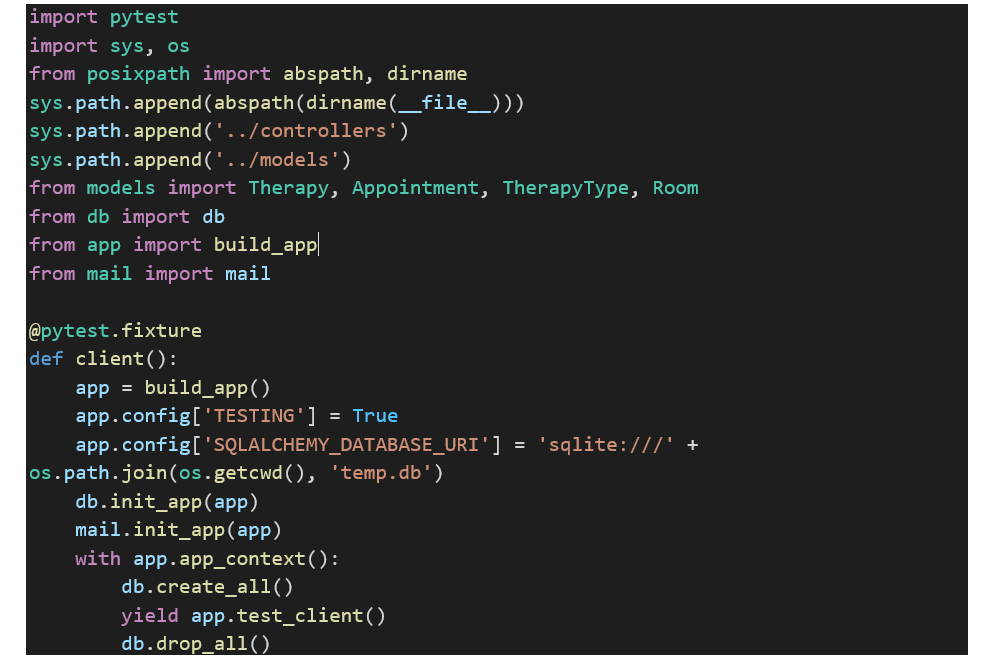
\includegraphics[scale=0.3]{slike/testno_okruzenje.PNG} %veličina slike u odnosu na originalnu datoteku i pozicija slike
				\centering
				\caption{Inicijalizacija testnog okruženja}
				\label{fig:testno_okruzenje}
			\end{figure}
			
			U prvom dijelu se definiraju korišteni moduli, a drugom dijelu se definira funkcija \textit{client} koja vraća instancu poslužitelja koju je onda moguće koristiti za testiranje. U funkciji se stvara prazna privremena baza podataka na istoj memorijskoj lokaciji. \\
S naredbama \texttt{db.init\_app(app)} će se inicijalizirati baza podataka po uzoru na db objekt koji sadrži sve entitete u poslužitelju. \texttt{mail.init\_app(app)} služi kako bi se omogućilo slanje obavijesti na e-poštu. Iako se ono ne provjerava tijekom testiranja, potrebno je za ispravan rad aplikacije. \\
Ova funkcija će se pokrenuti prije svakog testa kako bi se baza podataka očistila i time testovi ne bi utjecali jedni na druge.


\textbf{Testovi}


U testovima će se uglavnom testirati manipulacija terminima jer je to najsloženija procedura.

            \begin{figure}[H]
				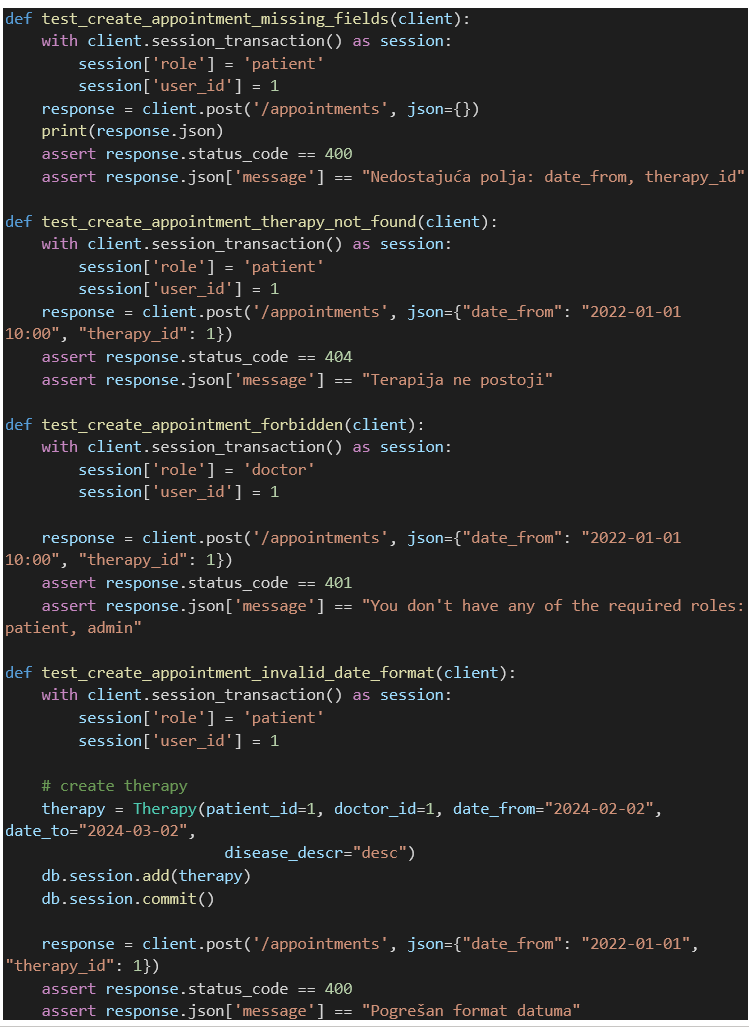
\includegraphics[scale=0.3]{slike/testovi_1_2_3_4.PNG} %veličina slike u odnosu na originalnu datoteku i pozicija slike
				\centering
				\caption{Testovi 1, 2, 3 i 4}
				\label{fig:testovi1234}
			\end{figure}
			
			\begin{figure}[H]
				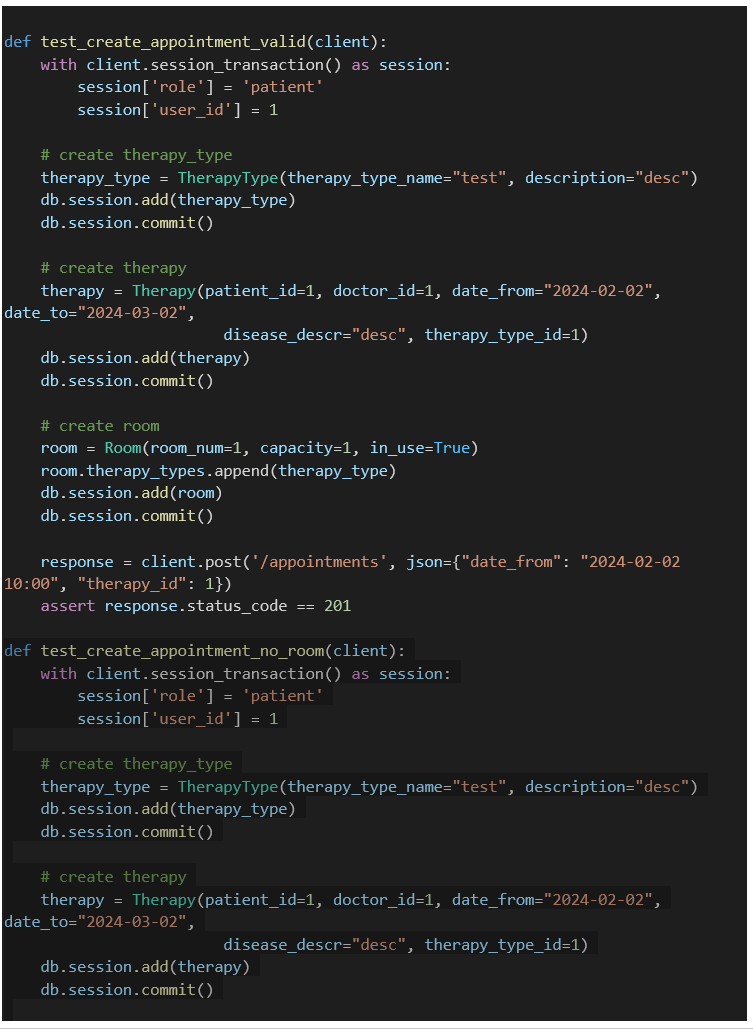
\includegraphics[scale=0.3]{slike/testovi_5_6dio.PNG} %veličina slike u odnosu na originalnu datoteku i pozicija slike
				\centering
				\caption{Testovi 5 i 6a}
				\label{fig:testovi56a}
			\end{figure}
			
			\begin{figure}[H]
				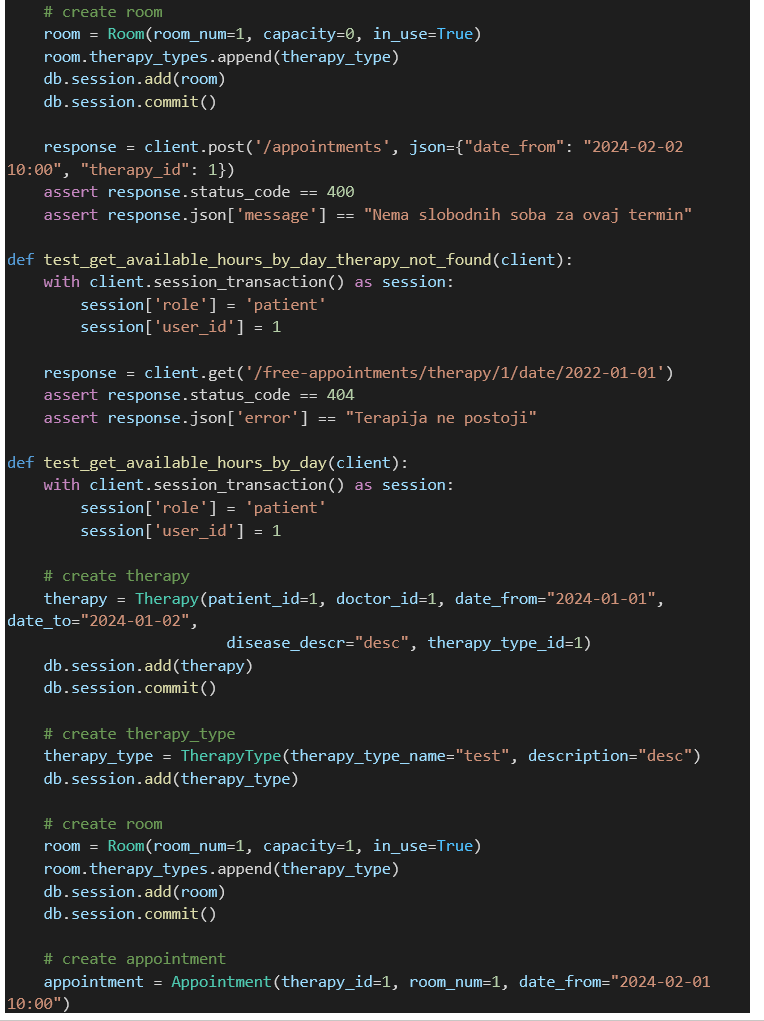
\includegraphics[scale=0.3]{slike/testovi_6dio_7_8dio.PNG} %veličina slike u odnosu na originalnu datoteku i pozicija slike
				\centering
				\caption{Testovi 6b, 7 i 8a}
				\label{fig:testovi6b78a}
			\end{figure}
			
			\begin{figure}[H]
				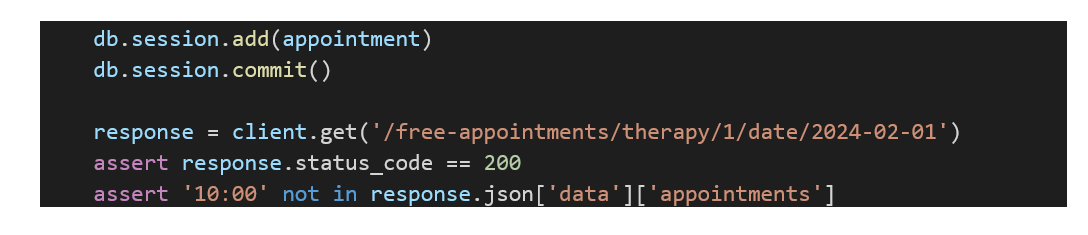
\includegraphics[scale=0.3]{slike/testovi_8dio.PNG} %veličina slike u odnosu na originalnu datoteku i pozicija slike
				\centering
				\caption{Test 8b}
				\label{fig:testovi8b}
			\end{figure}
			
			
	\begin{packed_item}
		\item \texttt{test\_create\_appointment\_missing\_fields(client)} \\
Testira hoće li funkcija za stvaranje termina (putem HTTP POST zahtjeva) vratiti status 400 i odgovarajuću poruku ako nedostaju polja \texttt{date\_from} i \texttt{therapy\_id}.
		\item \texttt{test\_create\_appointment\_therapy\_not\_found(client)} \\
		Provjerava hoće li funkcija vratiti status 404 i odgovarajuću poruku ako terapija s navedenim ID-jem ne postoji.
        \item \texttt{test\_create\_appointment\_forbidden(client)} \\
        Testira hoće li funkcija vratiti status 401 i odgovarajuću poruku ako korisnik koji pokušava stvoriti termin nema ulogu pacijenta ili administratora.
        \item \texttt{test\_create\_appointment\_invalid\_date\_format(client)} \\
        Provjerava hoće li funkcija vratiti status 400 i odgovarajuću poruku ako je format datuma neispravan prilikom stvaranja termina.
        \item \texttt{test\_create\_appointment\_valid(client)} \\
        Testira uspješno stvaranje termina (status 201) kada su svi uvjeti zadovoljeni, uključujući postojanje terapije, tipa terapije, sobe i slobodnih termina.	
        \item \texttt{test\_create\_appointment\_no\_room(client)}	\\
        	Provjerava hoće li funkcija vratiti status 400 i odgovarajuću poruku ako nema slobodnih soba za navedeni termin.
        \item \texttt{test\_get\_available\_hours\_by\_day\_therapy\_not\_found(client)} \\
        Testira hoće li funkcija za dobivanje slobodnih termina po danu vratiti status 404 i odgovarajuću poruku ako terapija s navedenim ID-jem ne postoji.
        \item texttt{test\_get\_available\_hours\_by\_day(client)} \\
        Provjerava ispravno dobivanje slobodnih termina (status 200) za određeni dan, uz pretpostavku da postoji terapija, tip terapije, soba i već stvoren termin na taj dan.
                   				
	 \end{packed_item}
	 
	 \textbf{Rezultati}
	 
	 
	 Svi testovi su usješno riješeni.
	 
	 \begin{figure}[H]
				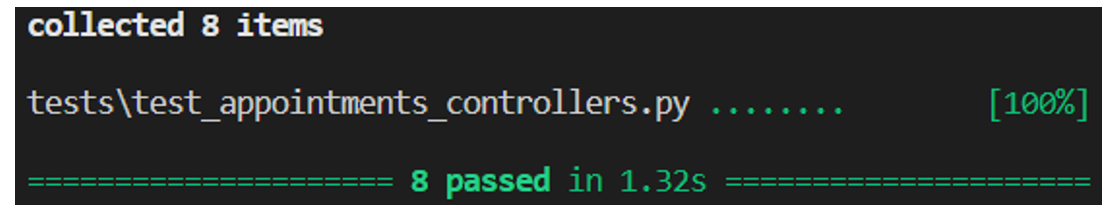
\includegraphics[scale=0.3]{slike/rezultati_testova.PNG} %veličina slike u odnosu na originalnu datoteku i pozicija slike
				\centering
				\caption{Rezultati testova}
				\label{fig:rezultati_testova}
			\end{figure}
	 
	 
			

			
			\subsection{Ispitivanje sustava}
			
			 \textit{Potrebno je provesti i opisati ispitivanje sustava koristeći radni okvir Selenium\footnote{\url{https://www.seleniumhq.org/}}. Razraditi \textbf{minimalno 4 ispitna slučaja} u kojima će se ispitati redovni slučajevi, rubni uvjeti te poziv funkcionalnosti koja nije implementirana/izaziva pogrešku kako bi se vidjelo na koji način sustav reagira kada nešto nije u potpunosti ostvareno. Ispitni slučaj se treba sastojati od ulaza (npr. korisničko ime i lozinka), očekivanog izlaza ili rezultata, koraka ispitivanja i dobivenog izlaza ili rezultata.\\ }
			 
			 \textit{Izradu ispitnih slučajeva pomoću radnog okvira Selenium moguće je provesti pomoću jednog od sljedeća dva alata:}
			 \begin{itemize}
			 	\item \textit{dodatak za preglednik \textbf{Selenium IDE} - snimanje korisnikovih akcija radi automatskog ponavljanja ispita	}
			 	\item \textit{\textbf{Selenium WebDriver} - podrška za pisanje ispita u jezicima Java, C\#, PHP koristeći posebno programsko sučelje.}
			 \end{itemize}
		 	\textit{Detalji o korištenju alata Selenium bit će prikazani na posebnom predavanju tijekom semestra.}
			
			\eject 
		
		
		\section{Dijagram razmještaja}
			
			 Specifikacijski dijagram razmještaja (\ref{fig:dijagram_razmjestaja1}) prikazuje kako se ključni dijelovi sustava razmještaju na fizičke i virtualne komponente te kako ti dijelovi međusobno komuniciraju.
			 Korisnik na svom računalu može s pomoću web preglednika pristupiti web aplikaciji. Oblak pruža poslužitelje za aplikaciju i bazu podataka. Korisničko računalo koje djeluje kao klijent komunicira s oblakom koje djeluje kao poslužitelj putem HTTP protokola. Web aplikacija i baza podataka također komuniciraju putem HTTP protokola.
			 
			 \begin{figure}[H]
				\includegraphics[scale=0.3]{slike/Dijagram_razmještaja_Aplikacija.PNG} %veličina slike u odnosu na originalnu datoteku i pozicija slike
				\centering
				\caption{Dijagram razmještaja}
				\label{fig:dijagram_razmjestaja1}
			\end{figure}
			
			\eject 
		
		\section{Upute za puštanje u pogon}
		
			\textbf{\textit{dio 2. revizije}}\\
		
			 \textit{U ovom poglavlju potrebno je dati upute za puštanje u pogon (engl. deployment) ostvarene aplikacije. Na primjer, za web aplikacije, opisati postupak kojim se od izvornog kôda dolazi do potpuno postavljene baze podataka i poslužitelja koji odgovara na upite korisnika. Za mobilnu aplikaciju, postupak kojim se aplikacija izgradi, te postavi na neku od trgovina. Za stolnu (engl. desktop) aplikaciju, postupak kojim se aplikacija instalira na računalo. Ukoliko mobilne i stolne aplikacije komuniciraju s poslužiteljem i/ili bazom podataka, opisati i postupak njihovog postavljanja. Pri izradi uputa preporučuje se \textbf{naglasiti korake instalacije uporabom natuknica} te koristiti što je više moguće \textbf{slike ekrana} (engl. screenshots) kako bi upute bile jasne i jednostavne za slijediti.}


\textbf{Postupak postavljanja baze podataka}

    \begin{packed_item}
		\item Postavljanje i konfiguracija PostgreSQL baze podataka unutar platforme Render \\
		
		U polje \textit{Name} potrebno je upisati ime instance PostgreSQL baze podataka. Polje \textit{Database} i \textit{User} Render popunjava s nasumično generiranim vrijednostima. Umjesto tih vrijednosti definirali smo vlastite, proginator za Database i proginator\_user za User. Nakon toga je potrebno odabrati regiju. Odabrali smo regiju Frankfurt (EU central) zato što je najbliža klijentu. 
		
		STAVI SLIKU!
		
		Nakon toga Render prikazuje informacije o bazi podataka: ime poslužitelja (\textit{Hostname}), vrata (\textit{Port}), ime baze podataka (\textit{Database}), korisničko ime PostgreSQL korisnika (\textit{username}), lozinku korisnika (\textit{password}) i URL za povezivanje na bazu podataka. 
		
		
		\item Konfiguracija pristupa bazi podataka iz aplikacije pgAdmin \\
		Unutar aplikacije pgAdmin potrebno je u izborniku odabrati Servers -> Register.
		
		SLIKA 
		
		Nakon toga, potrebno je ispuniti formu s podacima za povezivanje na bazu podataka koje smo dobili u platformi Render.
		SLIKA
		
		
        \item Incijalizacija baze podataka i stvaranje tablica \\

                   				
	 \end{packed_item}


\textbf{Postupak postavljanja backend aplikacije}

\begin{packed_item}
        \item Povezivanje Render web servisa s GitHub repozitorijem \\
  SLIKA 
        
         Render web servis povezujemo s GitHub repozitorijem kako bi Render platforma imala pristup izvornom kodu.
         
        \item Konfiguracija web servisa \\
        
        SLIKA
        \item Postavljanje varijabli okruženja
        
        SLIKA	
\end{packed_item}

\textbf{Postupak postavljanja frontend aplikacije}

\begin{packed_item}
   \item Konfiguracija web servisa \\
   
   SLIKA
   
   Ostali koraci jednaki su koracima postupka postavljanja backend aplikacije.
\end{packed_item}
			
			 \textit{Dovršenu aplikaciju potrebno je pokrenuti na javno dostupnom poslužitelju. Studentima se preporuča korištenje neke od sljedećih besplatnih usluga: \href{https://aws.amazon.com/}{Amazon AWS}, \href{https://azure.microsoft.com/en-us/}{Microsoft Azure} ili \href{https://www.heroku.com/}{Heroku}. Mobilne aplikacije trebaju biti objavljene na F-Droid, Google Play ili Amazon App trgovini.}
			
			
			\eject 